% \documentclass[10pt, handout]{beamer}
\documentclass[10pt]{beamer}

\usepackage{newpxtext}
\usepackage{physics}
\usepackage{bbold}

\usefonttheme{professionalfonts}
\usefonttheme{serif}

\usetheme{Pittsburgh}
\usecolortheme{beaver}

\setbeamertemplate{frametitle}[default][left]
\setbeamertemplate{navigation symbols}{}

\newcommand{\source}[1]{\begin{textblock*}{6cm}(0.5cm,8.8cm)
    \begin{beamercolorbox}[ht=0.5cm,left]{framesource}
        \usebeamerfont{framesource}\usebeamercolor[fg]{framesource} Source: {#1}
    \end{beamercolorbox}
\end{textblock*}}

\title{1D Chain of \\Majorana Fermions}
\author{Anthony REY}
\institute{\'Ecole Polytechnique Fédérale de Lausanne}
\date{\today}

\begin{document} % --------------------

\frame{\titlepage}

\begin{frame}
    \frametitle{Introduction}

    $\longrightarrow$ \textbf{O'Brien and Fendley} (2018) introduced a model with Tricritical Ising (TCI) point with supersymmetry exhibited on the lattice
    \vspace{1cm}

    \pause
    \begin{block}{Goal}
        Recover their phase diagram 
    \end{block}
    
    \pause
    \begin{block}{Method}
        Using DRMG, with open and periodic boundary conditions
    \end{block}

\end{frame}

\begin{frame}
    \frametitle{Model}
    
    Use O'Brien and Fendley (OF) model
    $$\mathcal{H} = 2\lambda_I \mathcal{H}_I + \lambda_3 \mathcal{H}_3 + \lambda_c \mathcal{H}_c$$\\
    with $$\begin{aligned} \mathcal{H}_I &= i \sum_a \gamma_a\gamma_{a+1} \xrightarrow{\text{JW}} -\sum_i \sigma^x_i\sigma^x_{i+1} + \sigma^z_i \\ \mathcal{H}_3 &= - \sum_a \gamma_{a-2}\gamma_{a-1}\gamma_{a+1}\gamma_{a+2} \xrightarrow{\text{JW}} \sum_i \sigma^z_i\sigma^x_{i+1}\sigma^x_{i+2} + \sigma^x_i\sigma^x_{i+1}\sigma^z_{i+2} \\ \mathcal{H}_c &= -i \sum_a \gamma_a\gamma_{a+2} \xrightarrow{\text{JW}} \sum_i \sigma^x_i\sigma^y_{i+1} - \sigma^y_i\sigma^x_{i+1} \end{aligned}$$
    where 
    \begin{itemize}
        \item JW is Jordan-Wigner transformation
        \item $\gamma_a$ is a Majorana fermion operator satisfying $\gamma_a = \gamma_a^\dagger$ and Clifford algebra $\{\gamma_a, \gamma_b\} = 2\delta_{ab}$
        \item from now on, $\lambda_c=0$
    \end{itemize}
\end{frame}

\begin{frame}
    \frametitle{Method}

    \begin{block}{Transverse-Field Ising}
        \begin{itemize}
            \item TFI model $$\mathcal{H} = -J\sum_i \sigma^x_i \sigma^x_{i+1} - h\sum_i \sigma^z_i$$
            \pause
            \item Described by CFT with central charge $c= \frac{1}{2}$ at criticality $|J| = |h|$
        \end{itemize}
    \end{block}

    \pause
    \begin{block}{Central charge}
        For OBCs, entanglement entropy given by Cardy-Calabrese formula $$S(\ell) = \frac{c}{6} \ln\left[\frac{2L}{\pi} \sin \frac{\pi \ell}{L} \right] + \text{const}$$ on bond $\ell$ for system of length $L$
    \end{block}
\end{frame}

\begin{frame}
    \frametitle{Results -- free OBCs}

    \begin{columns}
        \begin{column}{0.57\linewidth}
            \begin{figure}
                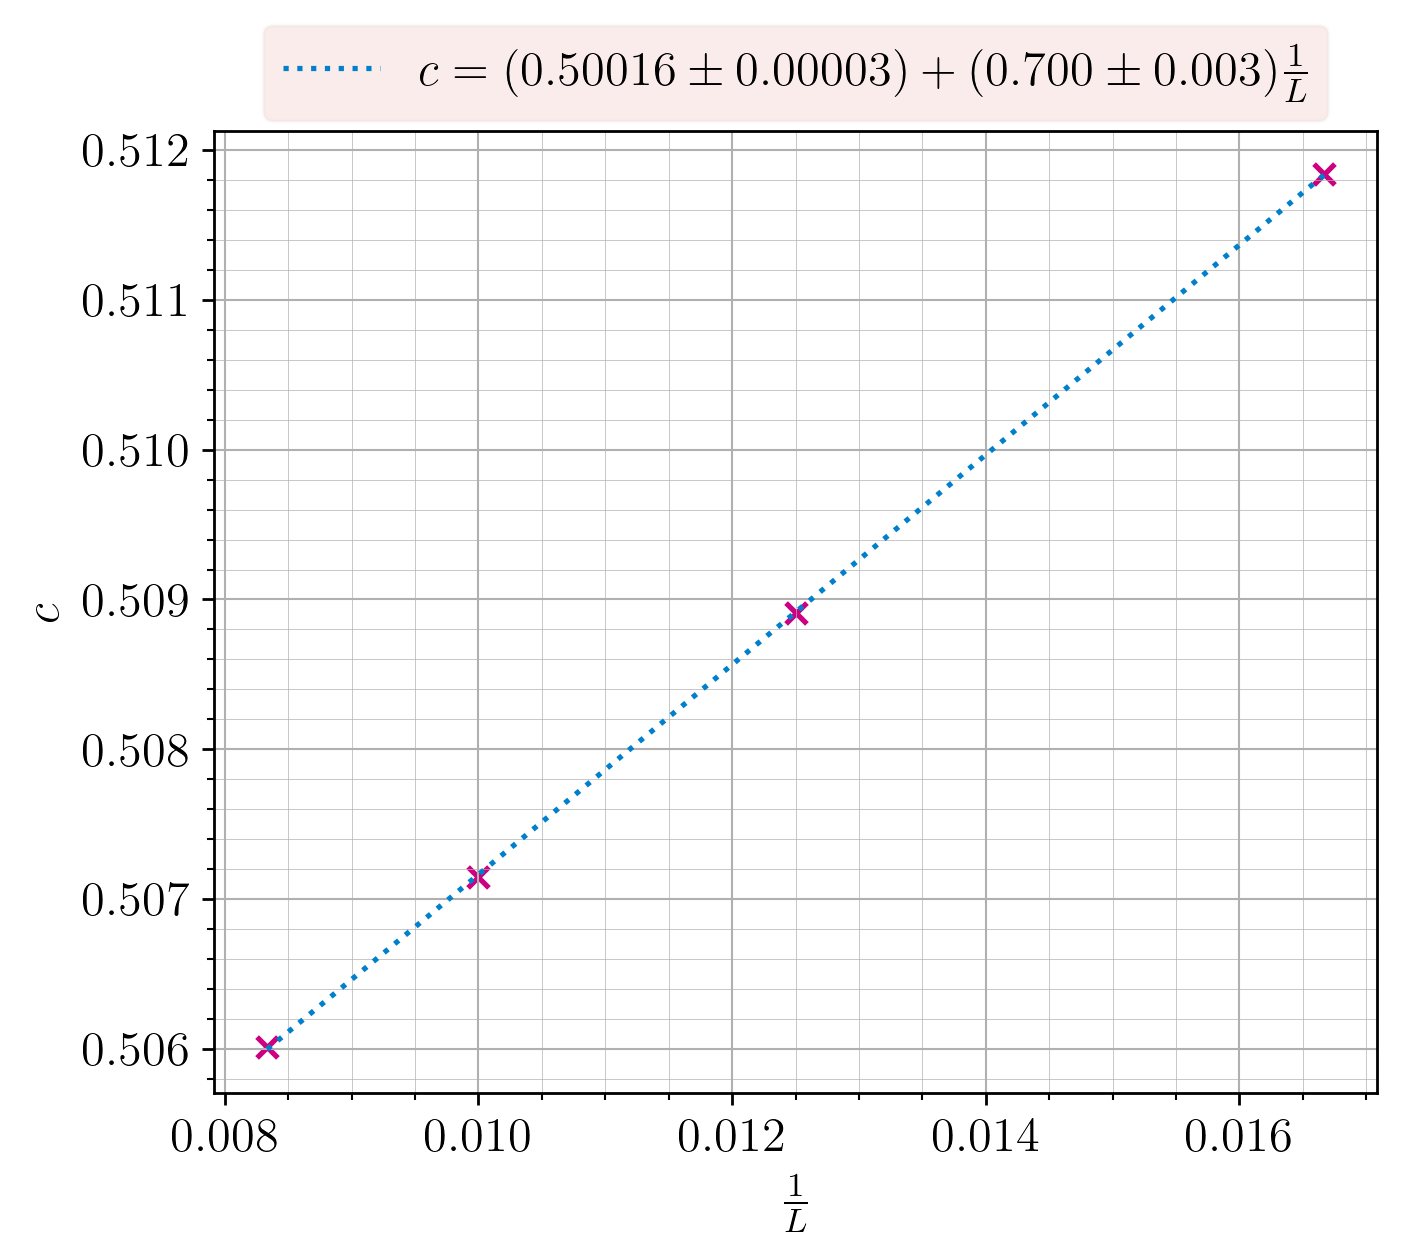
\includegraphics[scale=0.43]{../../graphs/entropies/ff/calabrese_chi=100.0_J=1.0_h=1.0_i=1.0_3=0.0_c=0.0.png}
                \caption{TFI with $J=h$, $\chi=100$}
            \end{figure}
        \end{column}

        \pause
        \begin{column}{0.6\linewidth}
            \begin{figure}
                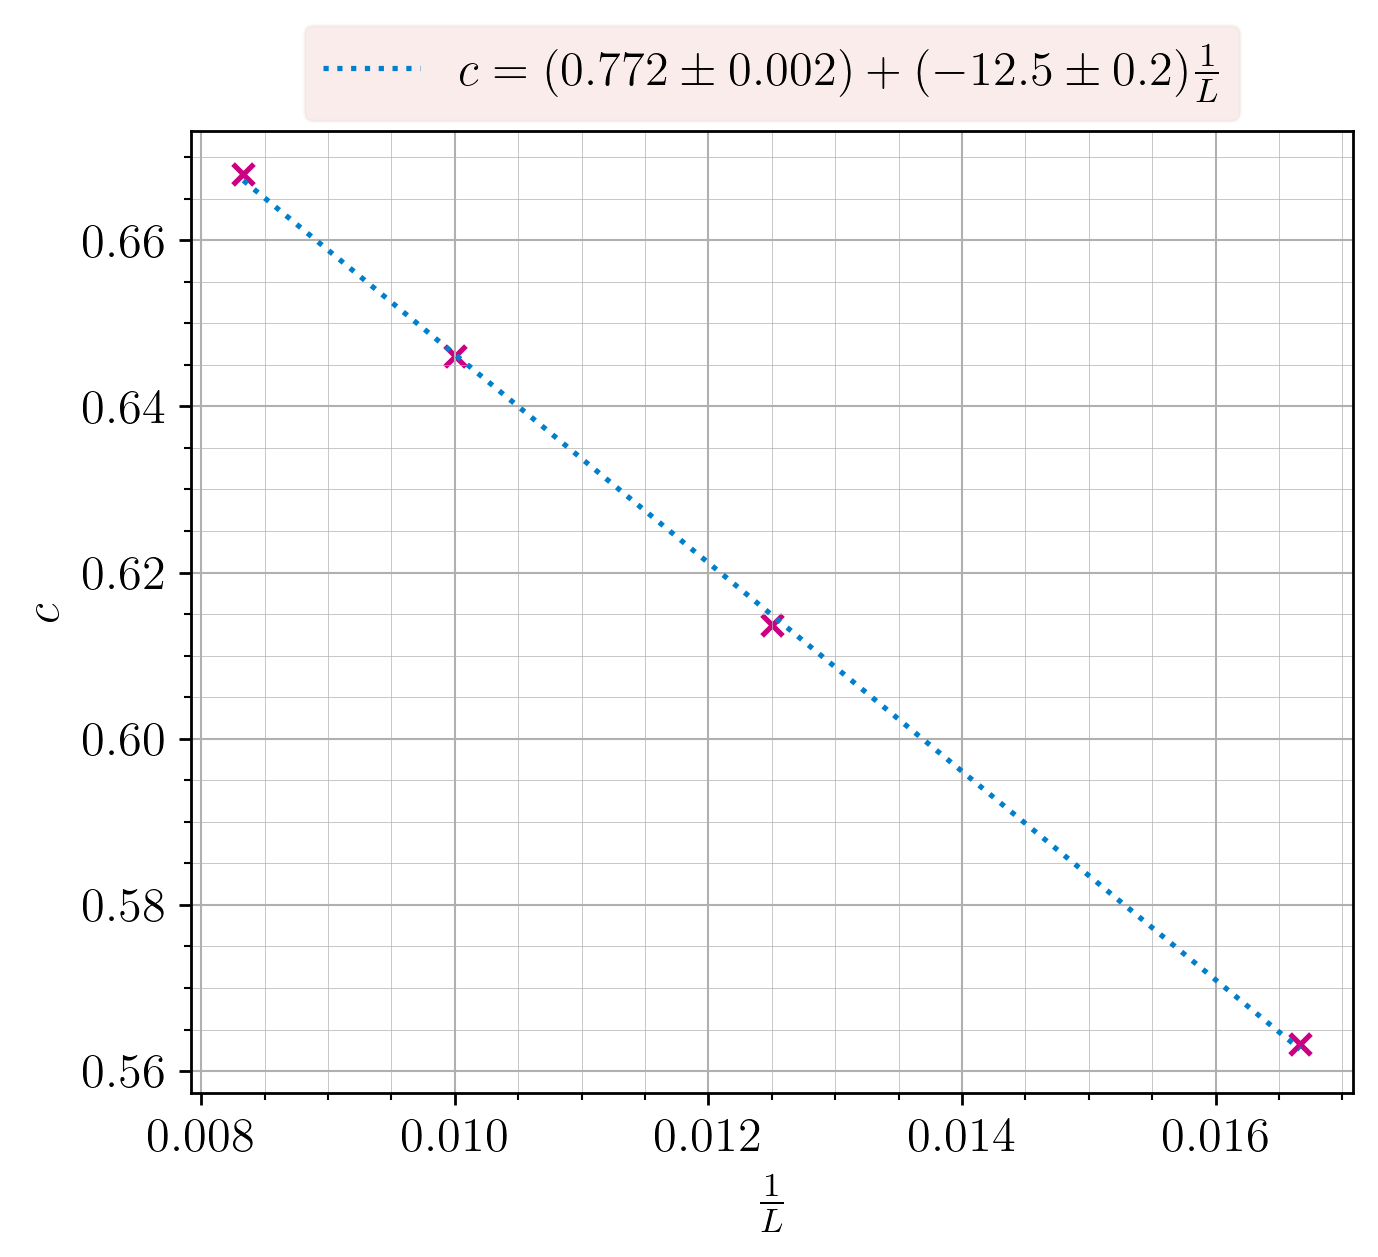
\includegraphics[scale=0.43]{../../graphs/entropies/ff/calabrese_chi=100.0_J=1.0_h=1.0_i=1.0_3=0.856_c=0.0.png}
                \caption{OF with $\lambda_3/\lambda_I =0.856$, $\chi=100$}
            \end{figure}
        \end{column}        
    \end{columns}
\end{frame}

\begin{frame}
    \frametitle{Results -- free OBCs}

    \begin{columns}
        \begin{column}{0.35\linewidth}
            \begin{block}{OF model}
                \begin{itemize}
                    \item is in Ising CFT for $\lambda_3/\lambda_I \in [0, 0.856[$ $\implies c=1/2$
                    \pause
                    \item is in TCI CFT for $\lambda_3/\lambda_I \simeq 0.856$ $\implies c=7/10$
                    \pause
                    \item is gapped for $\lambda_3/\lambda_I > 0.856$ $\implies c=0$
                \end{itemize}
            \end{block}
        \end{column}        

        \pause
        \begin{column}{0.75\linewidth}
            \begin{figure}
                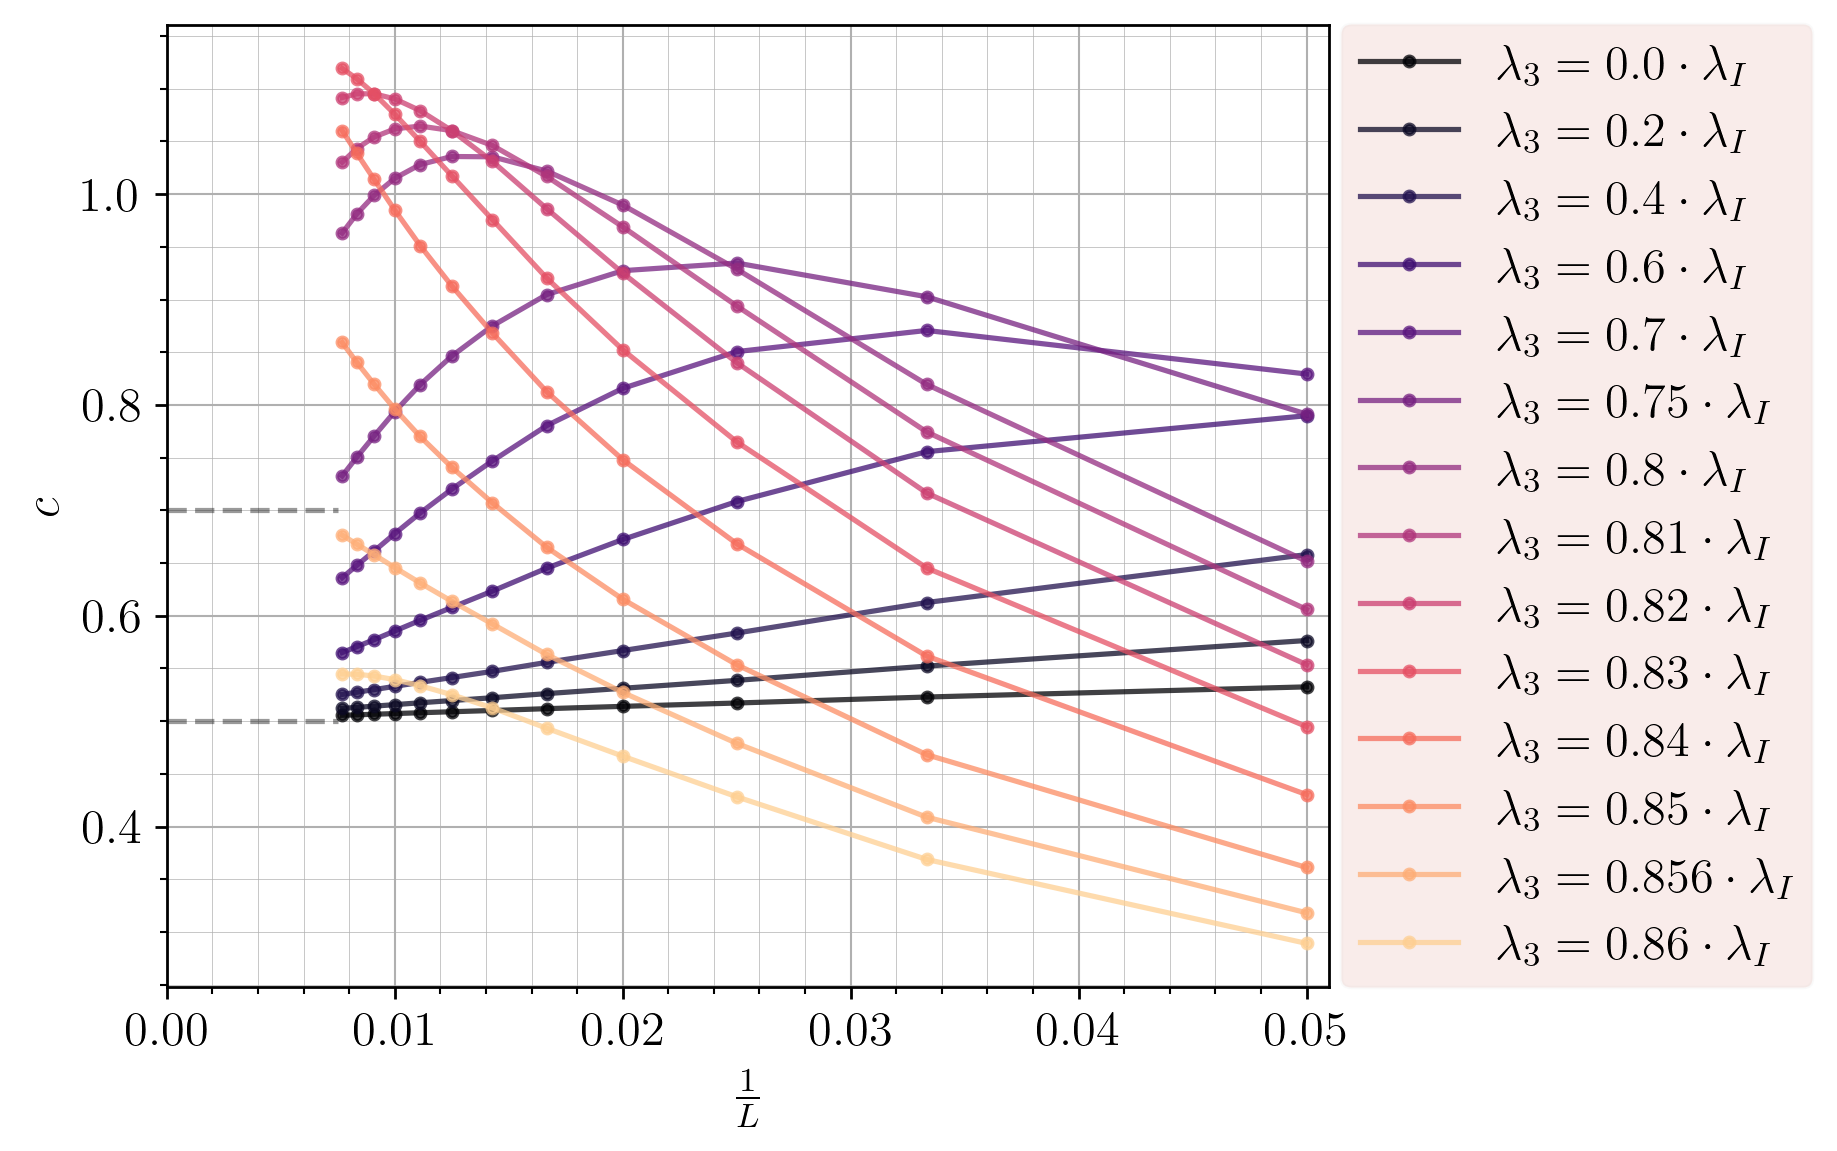
\includegraphics[scale=0.43]{../../graphs/phase/ff/chi=100.0_J=1.0_h=1.0_i=1.0_c=0.0.png}
                \caption{OF with $\lambda_3/\lambda_I$ varied, $\chi=100$}
            \end{figure}
        \end{column}
    \end{columns}
\end{frame}

\begin{frame}
    \frametitle{Results -- fixed OBCs}

    \begin{columns}
        \begin{column}{0.4\linewidth}
            \begin{block}{Problem}
                \begin{itemize}
                    \item Extrapolates to $0.772$ instead of $0.7$ !
                    \pause
                    \item Strange behavior for as we approach $\lambda_3/\lambda_I \simeq 0.856$
                \end{itemize}
            \end{block}

            \pause
            \begin{block}{Solution ?}
                \begin{itemize}
                    \item Try to pin edge spins in $x$-direction to reduce entropy in bulk
                    \pause
                    \item Results very good for critical TFI, allow to build conformal towers
                    \pause
                    \item But results even worse for TCI point
                \end{itemize}
            \end{block}
        \end{column}        

        \pause
        \begin{column}{0.6\linewidth}
            \begin{figure}
                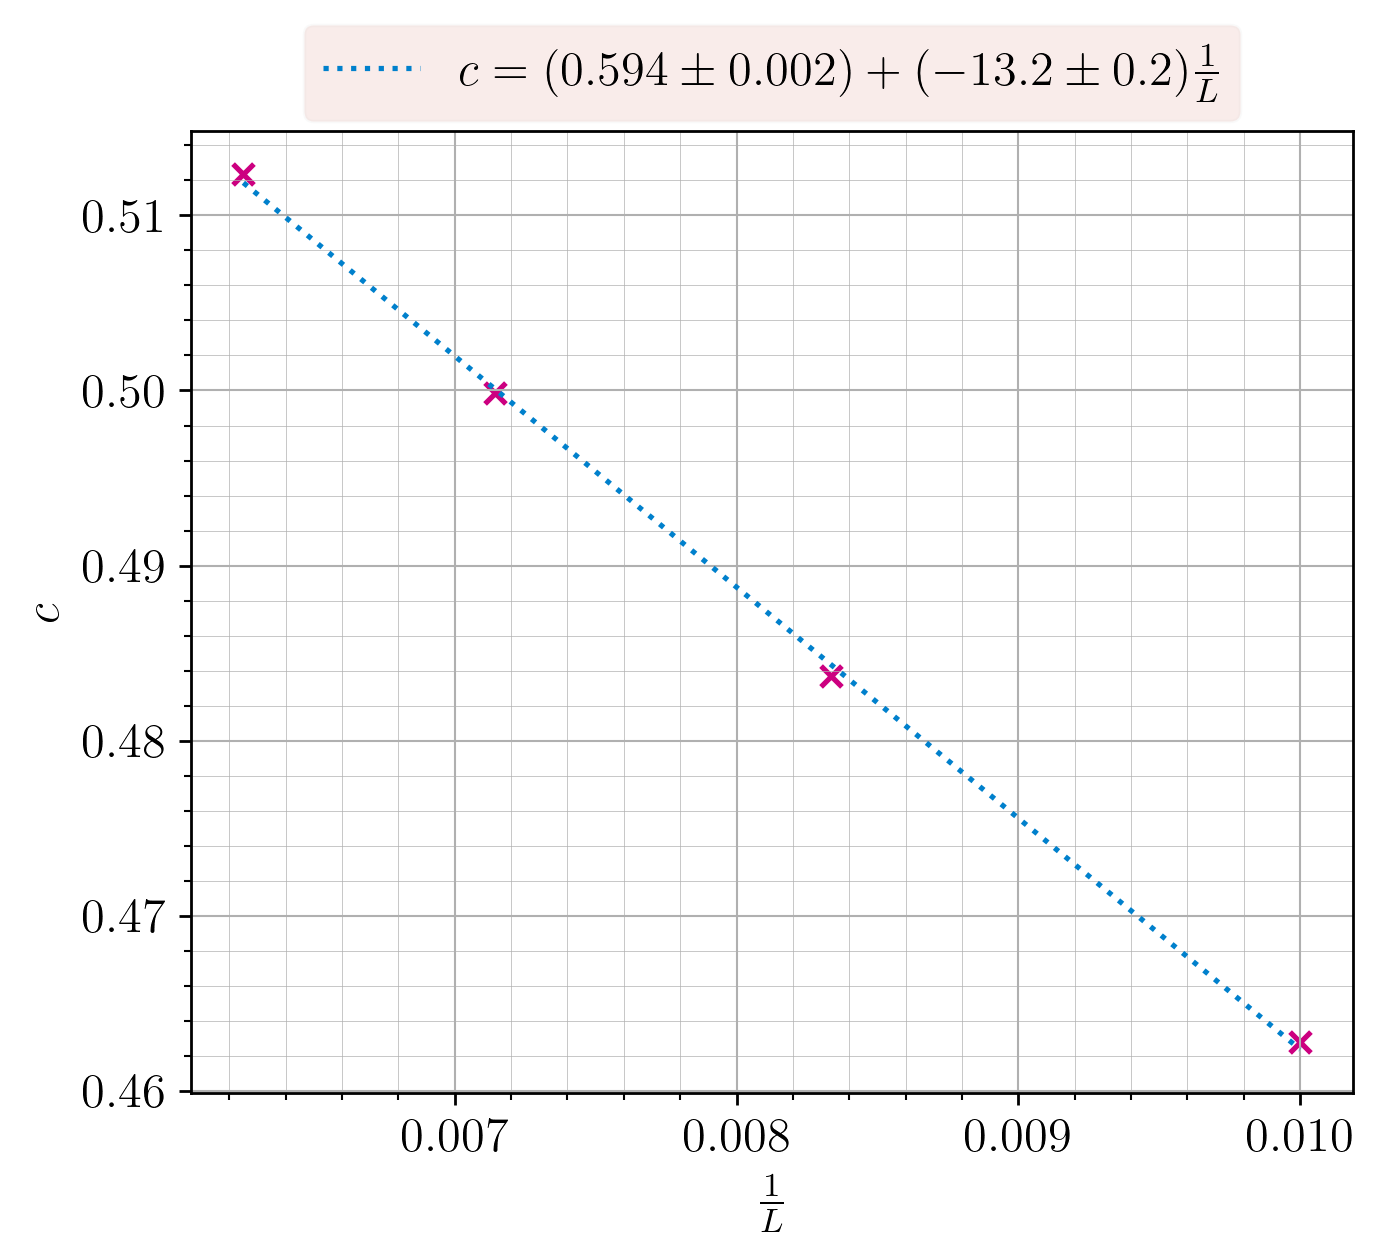
\includegraphics[scale=0.43]{../../graphs/entropies/--/100/calabrese_J=1.0_h=1.0_i=1.0_3=0.856_c=0.0.png}
                \caption{OF with $\lambda_3/\lambda_I = 0.856$, $\chi=100$ and $h_\text{pin} = -100$ ($[++]$ BCs)}
            \end{figure}
        \end{column}
    \end{columns}
\end{frame}

\begin{frame}
    \frametitle{Results -- PBCs}

        \begin{itemize}
            \item Expect to resolve the problem of central charge
            \pause
            \item Use another representation of the MPS 
                \begin{figure}
                    \hspace{-1cm}
                    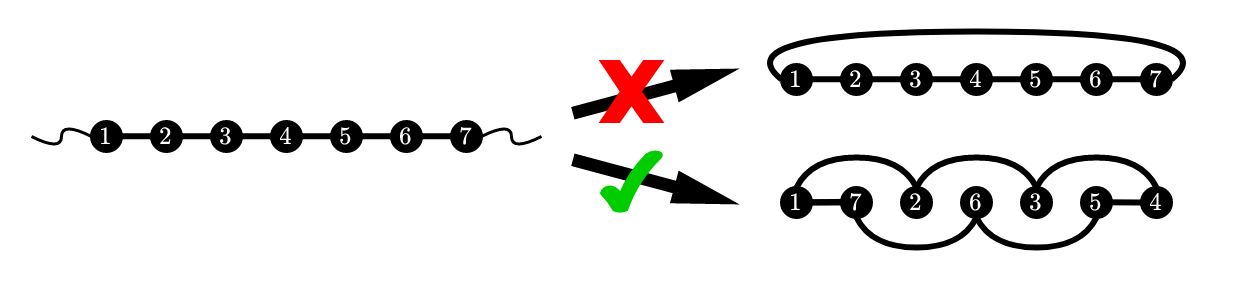
\includegraphics[scale=0.25]{../../images/pbcmps.png}
                \end{figure}
            \pause
            \item For PBCs, central charge recovered by $$S(\ell) = \frac{c}{3} \ln\left[\frac{L}{\pi} \sin \frac{\pi \ell}{L} \right] + \text{const}$$
        \end{itemize}
\end{frame}

\begin{frame}
    \frametitle{Results -- PBCs}

    \begin{columns}
        \begin{column}{0.55\linewidth}
            \begin{figure}
                \hspace{-0.8cm}
                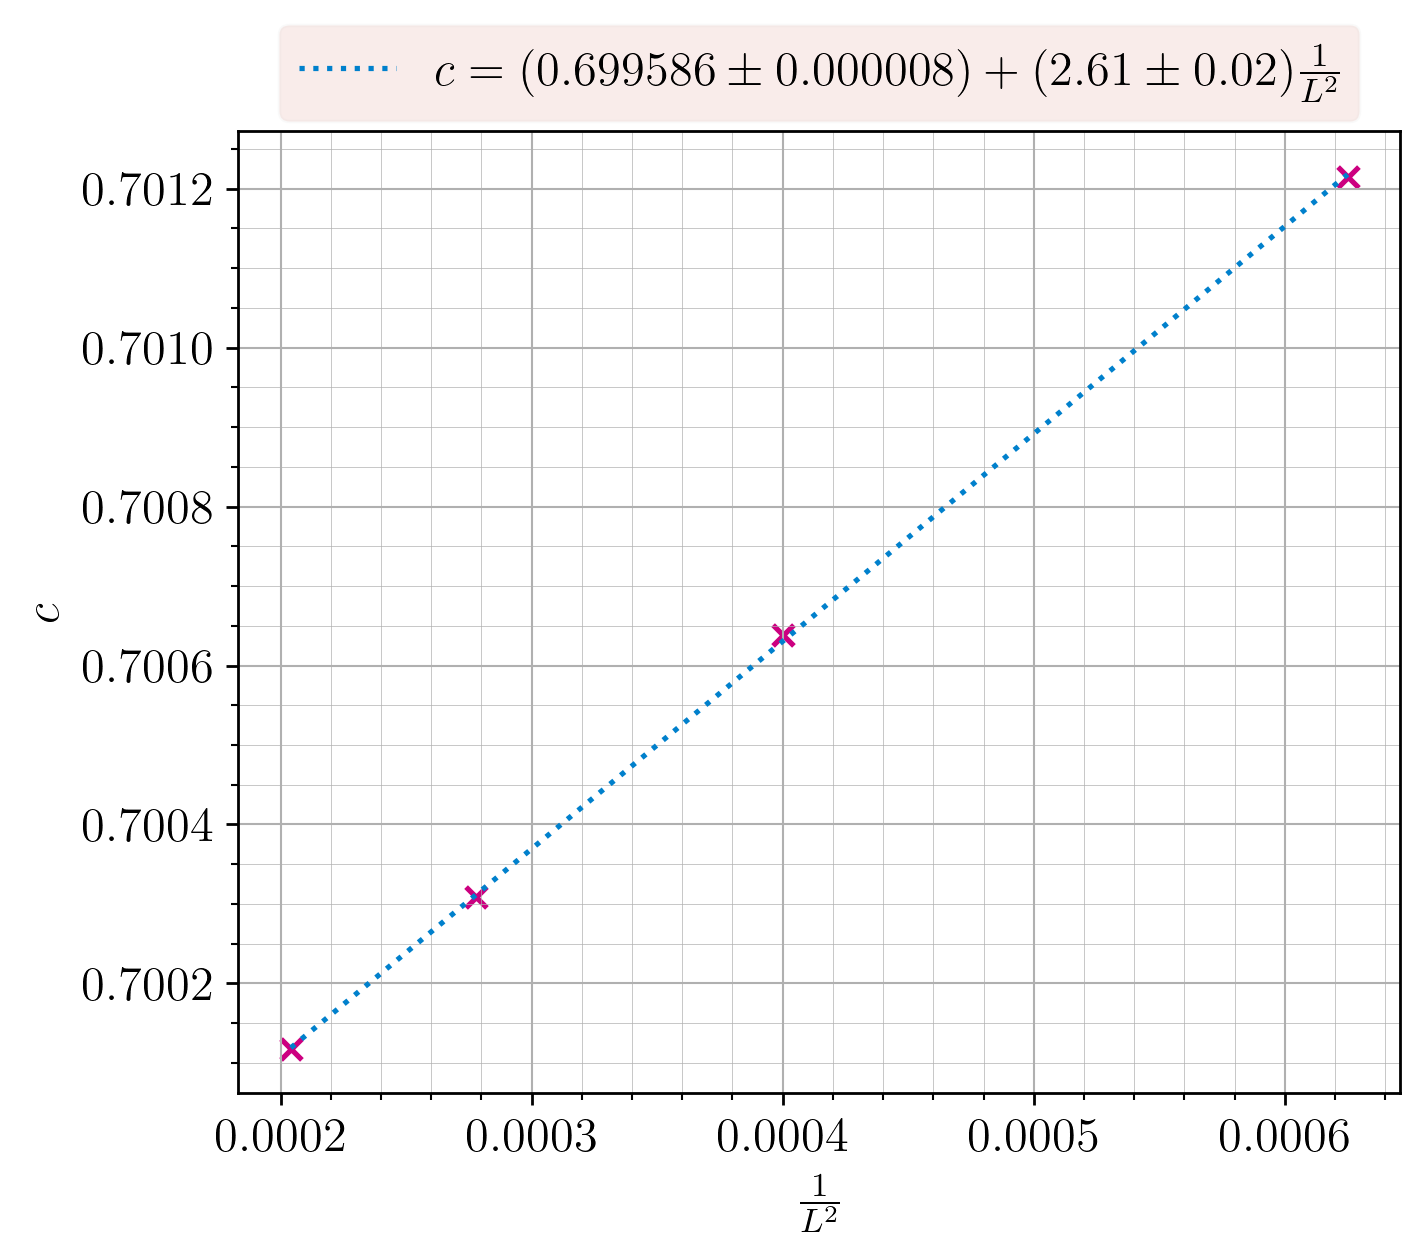
\includegraphics[scale=0.43]{../../graphs/entropies/pbc/10-4/calabrese_J=1.0_h=1.0_i=1.0_3=0.856_c=0.0.png}
                \caption{OF with $\lambda_3/\lambda_I=0.856$ and variance $\sim 10^{-4}$}
            \end{figure}
        \end{column}

        \pause
        \begin{column}{0.5\linewidth}
            \vspace{0.5cm}
            \begin{figure}
                \hspace{-0.8cm}
                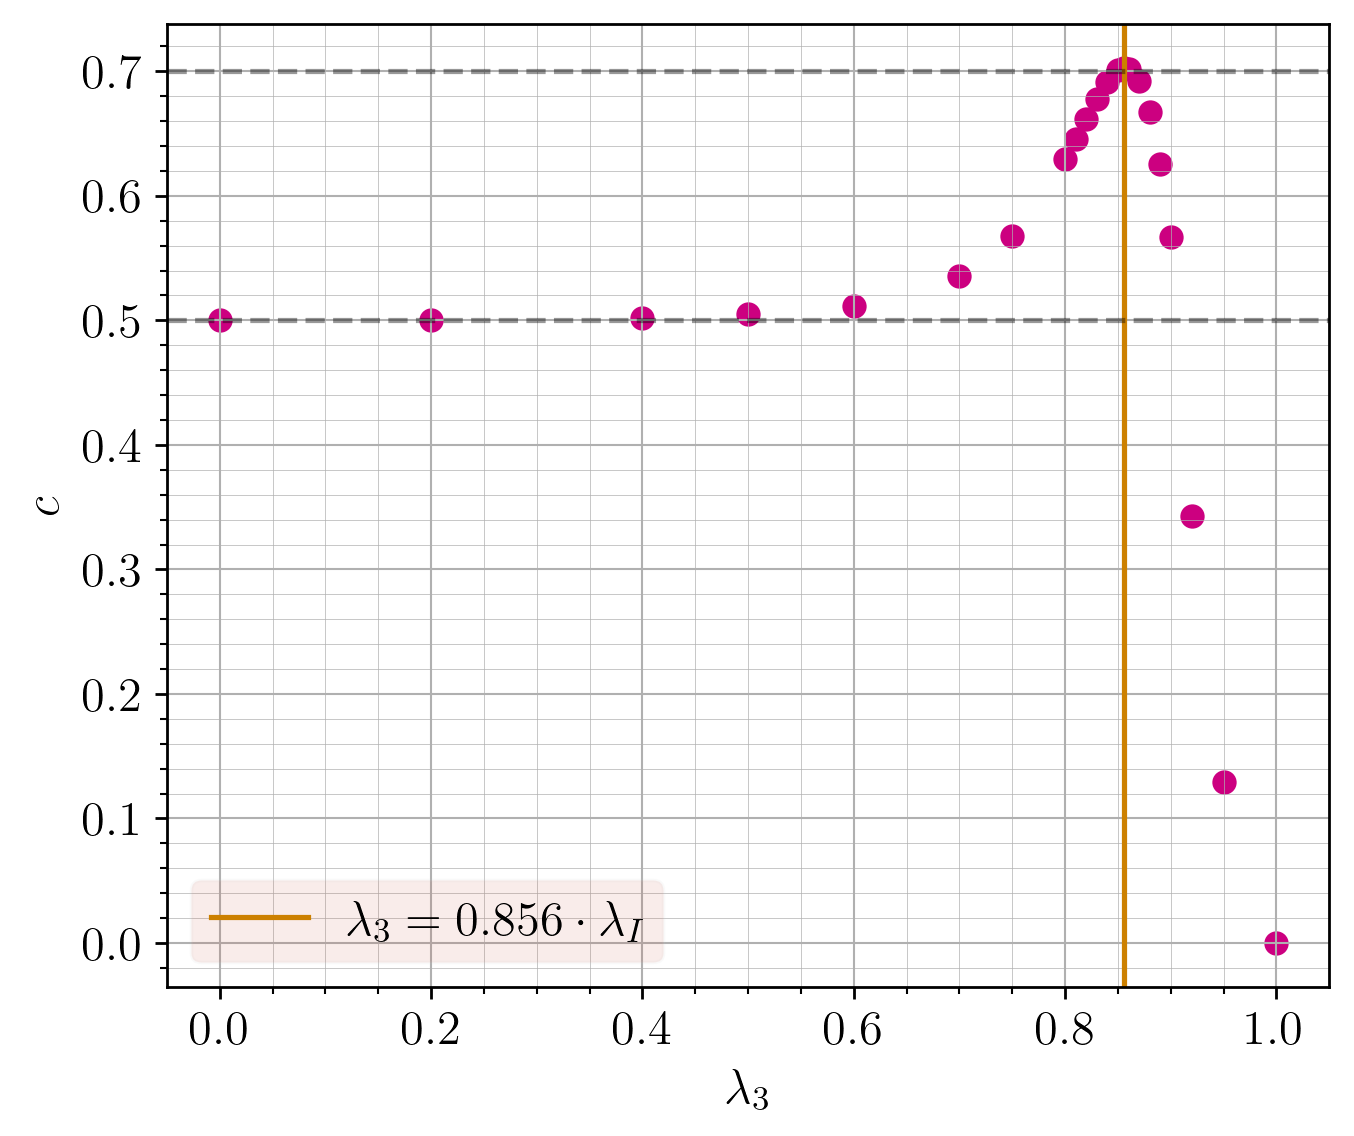
\includegraphics[scale=0.43]{../../graphs/through/pbc/L=30.0_chi=100.0_J=1.0_h=1.0_i=1.0_c=0.0.png}
                \caption{OF with $\lambda_3/\lambda_I$ varied, $L=30$ and $\chi=100$}
            \end{figure}
        \end{column}        
    \end{columns}
\end{frame}

\begin{frame}
    \frametitle{Results -- Ratios}

    \begin{block}{Excitation energies}
        \begin{itemize}
            \item Get excited energies directly through diagonalization of the effective Hamiltionian in 2-site update
            \pause
            \item Works perfectly at least for TFI where gap is correct and can build conformal towers with more than $10$ energies
        \end{itemize}
    \end{block}

    \pause
    \begin{block}{Parity}
        \begin{itemize}
            \item $\mathbb{Z}_2$-symmetry of Hamiltionian w.r.t. $\mathcal{F} = \prod_j \sigma^z_j$
            \pause
            \item Split $\mathcal{H}$ in sector with $\pm$ of $\mathcal{F}$, use projectors $\mathcal{F}^\pm = \frac{1}{2}[\mathbb{1} \pm \mathcal{F}]$ and run DMRG with $\tilde{\mathcal{H}} = \mathcal{F}^\pm \mathcal{H}\mathcal{F}^\pm $
        \end{itemize}
    \end{block}

    \pause
    \begin{table}
        \centering
        \renewcommand{\arraystretch}{1.3}
        \begin{tabular}{c|ccc}
            CFT & $R_1 = \frac{A^-_0 - P^+_0}{P^+_1 - P^+_0}$ & $R_2 = \frac{P^-_0 - P^+_0}{P^+_1 - P^+_0}$ & $R_3 = \frac{P^-_1 - P^+_0}{P^+_1 - P^+_0}$ \\
            \hline
            Ising & $\frac{1}{2}$ & $\frac{1}{8}$ & $\frac{9}{8}$ \\
            TCI & $\frac{7}{2}$ & $\frac{3}{8}$ & $\frac{35}{8}$
        \end{tabular}
        \caption{Universal ratios of energy computed from corresponding CFT.}
    \end{table}
\end{frame}

\begin{frame}
    \frametitle{Results -- Ratios}

    \begin{figure}
        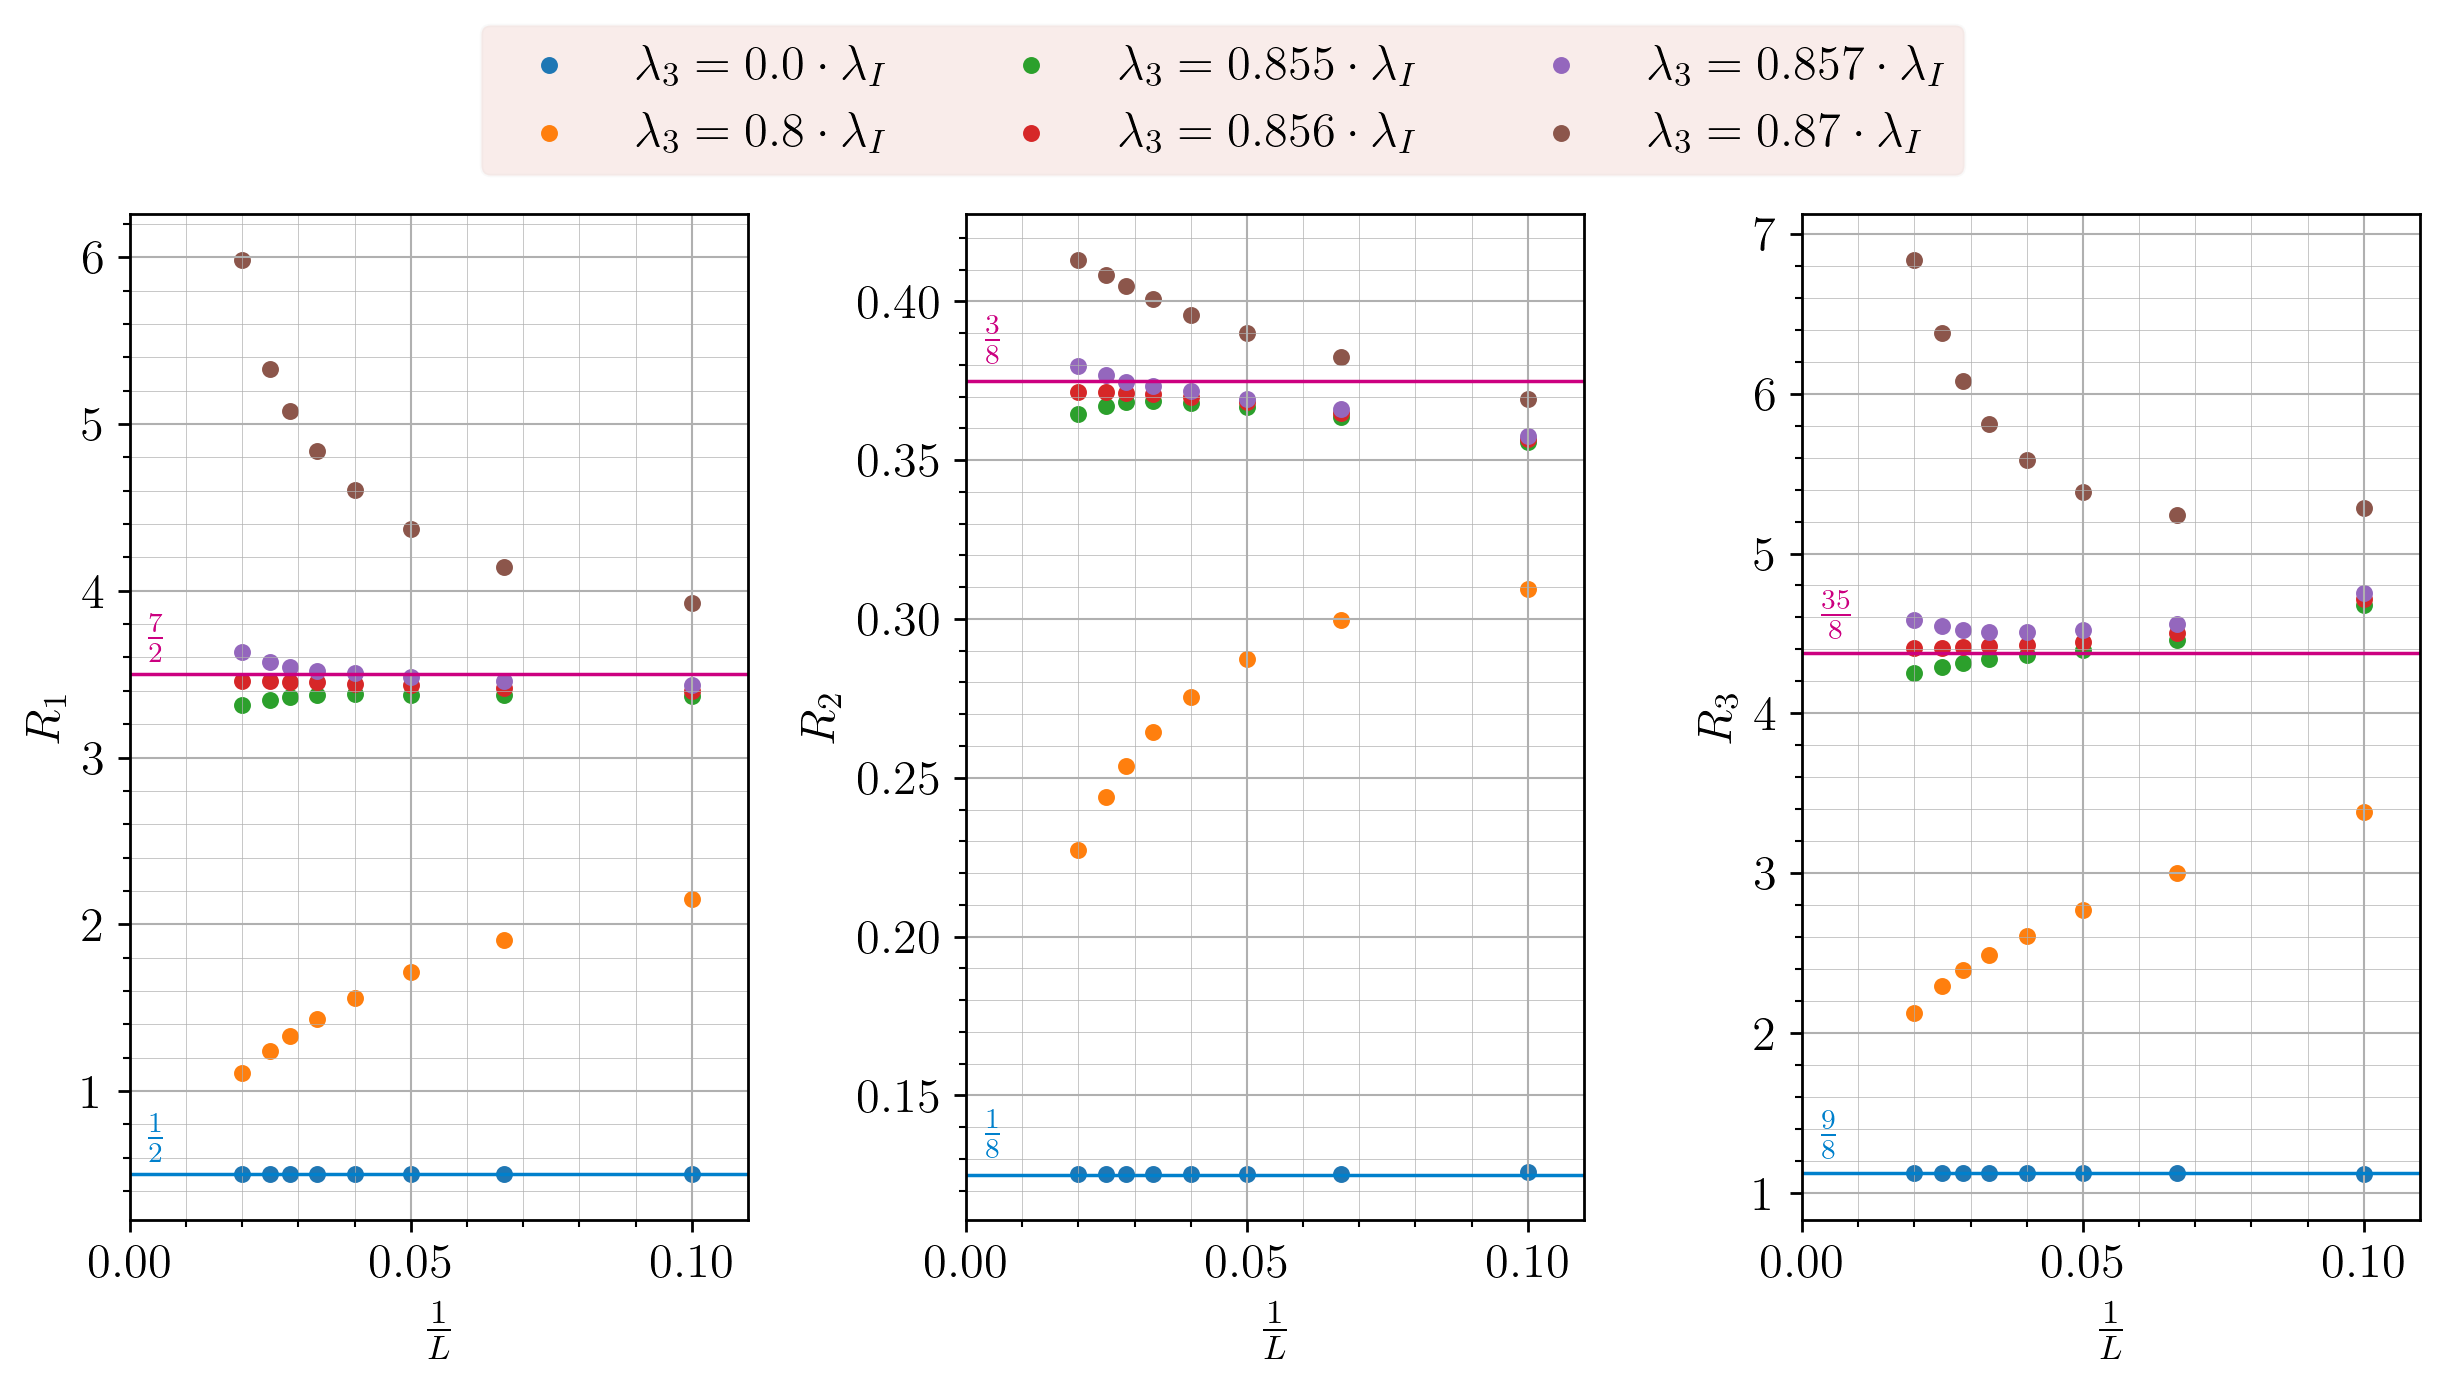
\includegraphics[scale=0.43]{../../graphs/ratios/J=1.0_h=1.0_i=1.0_c=0.0.png}
        \caption{Extrapolation of ratios with $\lambda_3/\lambda_I$ varied and variance $\sim 10^{-4}$}
    \end{figure}
\end{frame}

\begin{frame}
    \frametitle{Results -- Degeneracy in gapped phase}

    \begin{figure}
        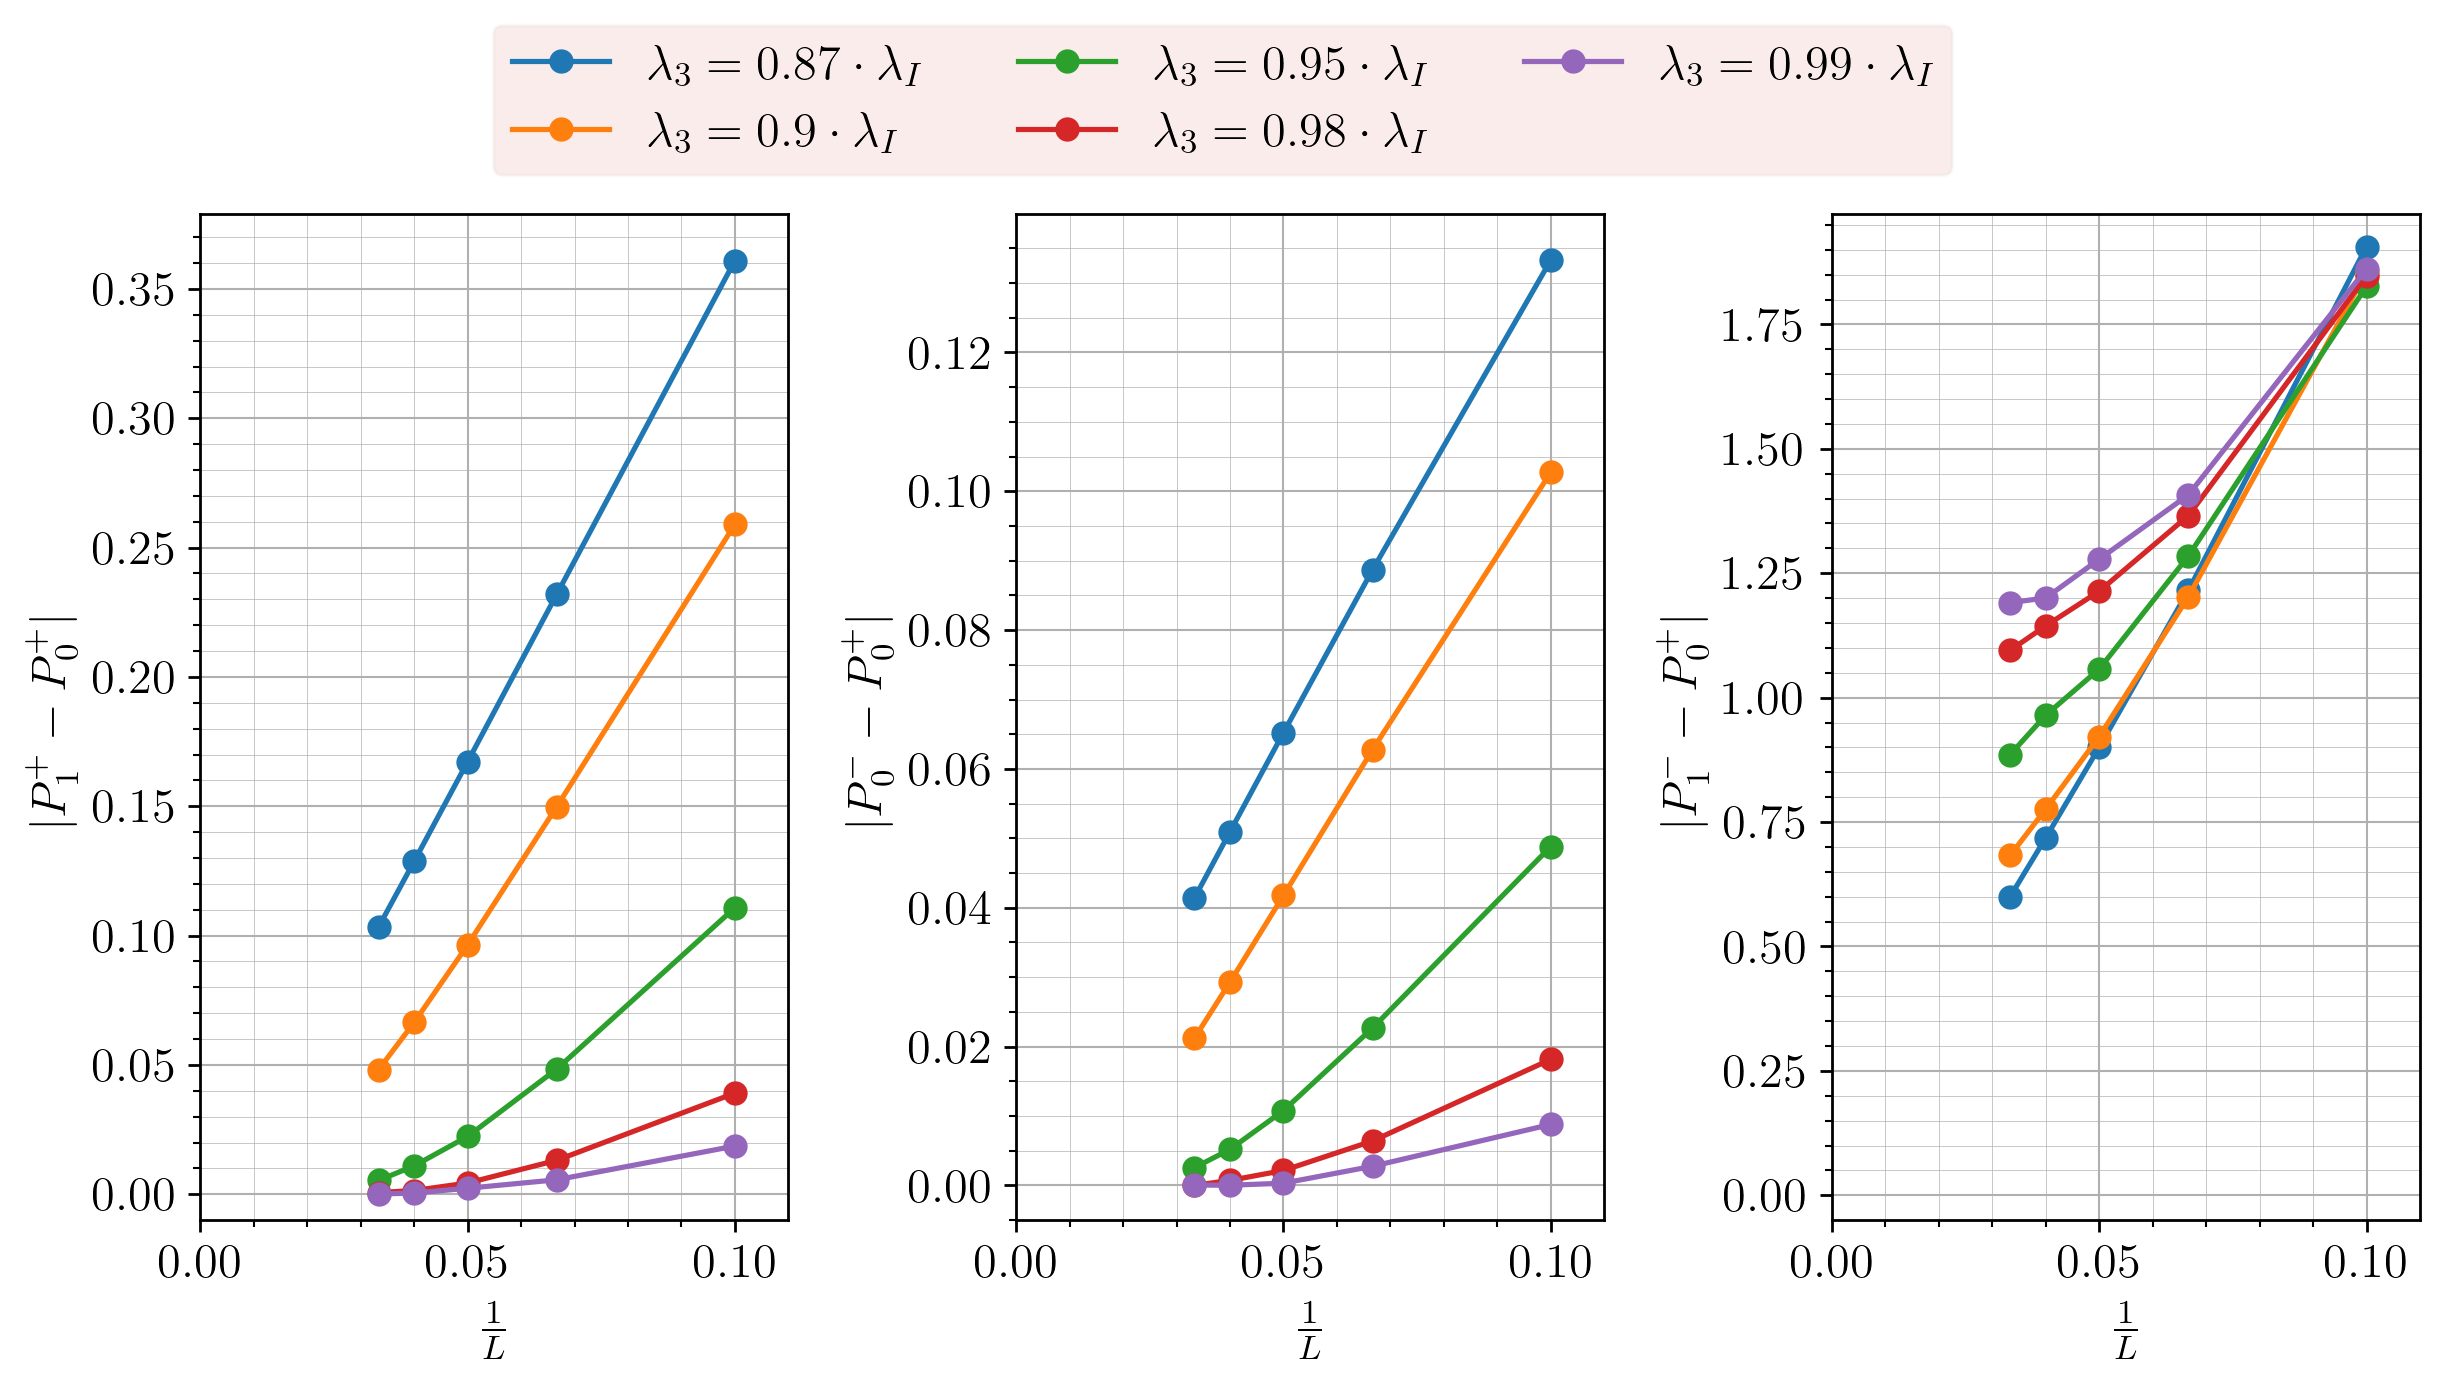
\includegraphics[scale=0.43]{../../graphs/degeneracy/J=1.0_h=1.0_i=1.0_c=0.0.png}
        \caption{Extrapolation of the differences in energies with $\lambda_3/\lambda_I >0.856$ varied and variance $\sim 10^{-4}$}
    \end{figure}
\end{frame}

\begin{frame}
    \frametitle{Conclusion}

    \begin{block}{Main achievements}
        \begin{itemize}
            \item Benchmark with TFI and description with Ising CFT
            \pause
            \item Phase diagram for OF model for $\lambda_3 \in [0, \lambda_I]$ and location of TCI CFT point at $\lambda_3/\lambda_I = 0.856$
        \end{itemize}
    \end{block}

    \pause
    \begin{block}{Further work}
        Introduce $\lambda_c \neq 0$ and complete phase diagram, but not done due to lack of because of struggles with TCI central charge
    \end{block}






\end{frame}

\end{document} % --------------------